%%%%%%%%%%%%%%%%%%%%%%%%%%%%%%%%%%%%%%%%%%%%%%%%%%
%% Luigi Marchionni
%% August 19 2013
%%%%%%%%%%%%%%%%%%%%%%%%%%%%%%%%%%%%%%%%%%%%%%%%%%

%%%%%%%%%%%%%%%%%%%%%%%%%%%%%%%%%%%%%%%%%%%%%%%%%% 
%% Begin Document
\documentclass[11pt]{article}


%%%%%%%%%%%%%%%%%%%%%%%%%%%%%%%%%%%%%%%%%%%%%%%%%% 
%%% Preamble
\usepackage{fullpage}
\usepackage{times}
\usepackage[colorlinks=TRUE, urlcolor=blue, citecolor=blue]{hyperref}
\usepackage[utf8]{inputenc}

%%% Additional packages
\usepackage{Sweave}
\usepackage{authblk}
\usepackage{color}
\usepackage[usenames, dvipsnames]{xcolor}

%%% Sweave options



%%%%%%%%%%%%%%%%%%%%%%%%%%%%%%%%%%%%%%%%%%%%%%%%%%
%%% New commands for R stuff
\newcommand{\software}[1]{\textsf{\texttt{#1}}}
\newcommand{\R}{\software{\bf R}}
\newcommand{\Bioc}{\software{Bioconductor}}
\newcommand{\Rcode}[1]{{\texttt{\color{BrickRed}{#1}}}}


%%%%%%%%%%%%%%%%%%%%%%%%%%%%%%%%%%%%%%%%%%%%%%%%%%
%%% Fancy Sweave
\DefineVerbatimEnvironment{Sinput}{Verbatim}{xleftmargin=1em, fontshape=sl, formatcom=\color{MidnightBlue}, fontsize=\footnotesize}
\DefineVerbatimEnvironment{Soutput}{Verbatim}{xleftmargin=1em,fontshape=sl,formatcom=\color{OliveGreen}, fontsize=\footnotesize}
\DefineVerbatimEnvironment{Scode}{Verbatim}{xleftmargin=1em,fontshape=sl,formatcom=\color{BrickRed}, fontsize=\footnotesize}
\fvset{listparameters={\setlength{\topsep}{0pt}}}
\renewenvironment{Schunk}{\vspace{\topsep}}{\vspace{\topsep}}


%%%%%%%%%%%%%%%%%%%%%%%%%%%%%%%%%%%%%%%%%%%%%%%%%%
%%% Begin document
\begin{document}
\Sconcordance{concordance:GeneSetAnalysis.tex:GeneSetAnalysis.Rnw:%
1 69 1 1 5 75 1 1 3 2 0 1 2 1 0 1 4 3 0 1 7 %
9 0 1 2 26 1 1 2 1 0 2 1 6 0 1 1 5 0 1 1 6 0 %
1 1 8 0 1 1 16 0 1 2 14 1 1 2 1 0 1 1 59 0 1 %
2 7 1 1 2 1 0 1 1 5 0 1 1 10 0 1 1 5 0 2 1 5 %
0 1 1 15 0 1 1 7 0 1 2 5 1 1 2 1 0 1 2 1 0 1 %
1 10 0 1 2 6 0 2 1 5 0 1 1 1 2 1 0 1 1 11 0 %
1 2 3 1 1 2 1 0 1 1 22 0 2 1 15 0 1 2 3 1 1 %
2 1 0 1 1 30 0 2 1 15 0 1 2 3 1 1 2 1 0 1 1 %
10 0 1 1 11 0 1 2 23 1 1 2 8 0 1 2 41 1 1 2 %
1 0 1 2 4 0 1 2 7 1 1 3 2 0 1 2 1 0 1 2 4 0 %
1 2 8 1 1 4 3 0 1 3 5 0 1 2 1 1 1 2 27 0 1 1 %
16 0 1 1 17 0 1 2 8 1 1 2 1 0 1 2 4 0 1 2 3 %
1 1 2 26 0 1 1 6 0 1 2 5 1 1 6 5 0 1 2 4 0 1 %
2 6 1 1 2 26 0 1 2 20 0 1 2 7 1 1 2 1 0 1 1 %
3 0 1 2 3 1 1 2 7 0 1 1 6 0 1 1 13 0 1 1 13 %
0 1 1 26 0 1 1 27 0 1 2 7 1 1 3 6 0 1 2 12 1 %
1 3 6 0 1 2 22 1 1 3 2 0 1 1 7 0 1 2 9 1 1 6 %
8 0 1 2 2 1 1 2 1 0 1 1 5 0 2 1 7 0 1 1 7 0 %
1 2 2 1 1 3 5 0 1 2 3 1 1 2 11 0 1 1 6 0 1 1 %
8 0 1 1 6 0 1 1 6 0 1 1 7 0 1 2 2 1 1 2 1 0 %
1 1 24 0 1 1 17 0 1 2 5 1 1 2 30 0 1 2 8 1}



%%%%%%%%%%%%%%%%%%%%%%%%%%%%%%%%%%%%%%%%%%%%%%%%%%
%%% Title of the document

\title{Reproducible Gene Set Analysis with R}

\author{Luigi Marchionni \\
Department of Oncology \\
Johns Hopkins University \\
email: \texttt{marchion@jhu.edu}}


%%%%%%%%%%%%%%%%%%%%%%%%%%%%%%%%%%%%%%%%%%%%%%%%%%
%%% Table of contents
\maketitle
\tableofcontents


%%%%%%%%%%%%%%%%%%%%%%%%%%%%%%%%%%%%%%%%%%%%%%%%%%
%%% Setting options, cleaning the workspace



%%%%%%%%%%%%%%%%%%%%%%%%%%%%%%%%%%%%%%%%%%%%%%%%%%
%%% Introductory considerations
\newpage
\section{Overview}
Gene Set Analysis (GSA) has been widely use to assist the interpretation
of results from gene expression and genomic data analyses.

In today's tutorial we will use {\R} to perform GSA using methods and examples
based on the \Rcode{RTopper} \cite{Tyekucheva2011} and \Rcode{limma} packages
\cite{Smyth2005a,Smyth2004,Smyth2005}.

In particular we will use example data and wrapper functions from \Rcode{RTopper}
in conjuction with the \Rcode{GeneSetTest} function from \Rcode{limma}, 
which enables testing the hypothesis that a specific set of genes
(a Functional Gene Set, FGS) is more highly ranked on a given statistics.
using the Wilcoxon rank-sum test. We will also illustrate alternative
strategies, creating user-defined functions based on the Fisher's exact test.
Overall, this approach is conceptually analogous to
Gene Set Enrichment Analysis (GSEA), as proposed by Mootha 
and colleagues \cite{Mootha2003a,Subramanian2005}.

In addition we will also show how to correct for multiple hypothesis by
applying the Benjamini and Hochberg method \cite{Benjamini1995}
as implemented in the \Rcode{multtest} R/Bioconductor package.

Finally we will also show where and how to retrieve FGS information, including
providing simple code to cross-reference common gene identifiers.
To achieve all these goals we will need to start by refreshinga few basic
\R commands and concepts.



%%%%%%%%%%%%%%%%%%%%%%%%%%%%%%%%%%%%%%%%%%%%%%%%%% 
%%%%%%%%%%%%%%%%%%%%%%%%%%%%%%%%%%%%%%%%%%%%%%%%%%
\section{{\R}-{\Bioc} analytical packages}

The following {\R} packages were used to perform our analyses
and produce this vignette:
\begin{itemize}
  \item \Rcode{BiocGenerics}: this library implements several generic 
    classes and methods to work with {\Bioc} packages 
    and can be obtained from {\Bioc};
  \item \Rcode{Biobase}: this library implements classes and methods 
    to work with genomic data and can be obtained from {\Bioc};
  \item \Rcode{limma}: this library provide advanced methods to perform
    gene expression analysis from raw data to gene set analysis
    and can be obtained from {\Bioc};
  \item \Rcode{RTopper}: this library implements methods to perform
    integrated gene set analysis across datasets and platforms
    and can be obtained from {\Bioc};
  \item \Rcode{multtest}: this library implements methods to perform
    multiple test correction and can be obtained from {\Bioc};
  \item \Rcode{org.Hs.eg.db}: this library contains human genes annotation
    and can be obtained from {\Bioc};
  \item \Rcode{KEGG.db}: this library contains KEGG pathway annotation
    and can be obtained from {\Bioc};
  \item \Rcode{reactome.db}: this library contains Reactome pathway annotation
    and can be obtained from {\Bioc};
  \item \Rcode{GO.db}: this library contains Gene Ontoogy annotation
    and can be obtained from {\Bioc};
  \item \Rcode{AnnotationDBI} and \Rcode{annotate}:
    these libraries contain classes and methods
    to access and manipulated annotation packages 
    and can be obtained from {\Bioc};
\end{itemize}    


\subsection{Install the packages}

The chunk of {\R} code below can be used to obtain and install 
all necessary packages from \texttt{CRAN}, {\Bioc}, or the website 
repository accompanying this manuscript.
Installing from {\Bioc}:

\begin{Schunk}
\begin{Sinput}
> ###Source the biocLite.R script from Bioconductor
> source("http://bioconductor.org/biocLite.R")
> ###Get the list of available packages
> installedPckgs <- installed.packages()[,"Package"]
> ###Define the list of desired libraries
> pckgListBIOC <- c("BiocGenerics", "Biobase", "limma", "RTopper", 
+ 		  "org.Hs.eg.db", "AnnotationDbi", "annotate", 
+ 		  "multtest", "KEGG.db", "GO.db")
> ###Load the packages, install them from Bioconductor if needed
> for (pckg in pckgListBIOC) {
+ 	if (! pckg %in% installedPckgs) {
+ 		biocLite(pckg, suppressUpdates=TRUE, ask=FALSE)
+ 		}
+ 	require(pckg, character.only=TRUE)
+ }
\end{Sinput}
\end{Schunk}

  

%%%%%%%%%%%%%%%%%%%%%%%%%%%%%%%%%%%%%%%%%%%%%%%%%% 
%%%
\section{Gene Set Analysis with RTopper}

\subsection{RTopper data structure}
In this tutorial we will use some of the functions of the \Rcode{RTopper} package.
To this end we will make use of simplified data generated within 
The Cancer Genome Atlas (TCGA) project,
using Glioblastoma Multiforme (GBM) genomics data obtained from the same
patients" cohort using distinct platforms, including Differential Gene Expression (DGE),
Copy Number Variation (CNV), and Differential Methylation (DM).
This data is included with the \Rcode{RTopper} package as the dataset \texttt{exampleData},
which consists of genomic measurements (the list \Rcode{dat}) 
for 500 genes (in rows) and 95 patients (in columns) from 4 distinct platforms:
\begin{enumerate}
  \item DGE obtained using Affymetrix;
  \item DGE obtained using Agilent;
  \item CNV data generated ad Harvard;
  \item CNV data generated ad the MSKCC;
\end{enumerate}

Load the data set type \Rcode{data(sepScores)}, and to view a description of this 
data type \Rcode{?sepScores}. The structure of the data is shown below:

\begin{Schunk}
\begin{Sinput}
> require(RTopper)
> data(sepScores)
> ls()
\end{Sinput}
\begin{Soutput}
[1] "installedPckgs" "pckg"          
[3] "pckgListBIOC"   "sepScores"     
\end{Soutput}
\begin{Sinput}
> class(sepScores)
\end{Sinput}
\begin{Soutput}
[1] "list"
\end{Soutput}
\begin{Sinput}
> names(sepScores)
\end{Sinput}
\begin{Soutput}
[1] "dat.affy"       "dat.agilent"   
[3] "dat.cnvHarvard" "dat.cnvMskcc"  
\end{Soutput}
\begin{Sinput}
> sapply(sepScores, class)
\end{Sinput}
\begin{Soutput}
      dat.affy    dat.agilent dat.cnvHarvard 
     "numeric"      "numeric"      "numeric" 
  dat.cnvMskcc 
     "numeric" 
\end{Soutput}
\begin{Sinput}
> sapply(sepScores,dim)
\end{Sinput}
\begin{Soutput}
$dat.affy
NULL

$dat.agilent
NULL

$dat.cnvHarvard
NULL

$dat.cnvMskcc
NULL
\end{Soutput}
\end{Schunk}


\subsection{Creation of Functional Gene Sets}
Functional Gene Sets (FGS) are list of genes that share a specific biological function.
Examples of FGS are genes that operate in the same signaling pathway 
({\it i.e.} Notch signaling genes), or that share the same biological function
({\it i.e.} Cell adhesion genes).
FGS can be retrieved from various database, or can be construncted {\it ad hoc}.
A convenient source of FGS are the R-Bioconductor metaData packages,
and S4 classes and methods for handling FGS are provided by the \Rcode{GSEABase}
package. Below is shown a simple way to extract FGS from the human genome
metaData package \Rcode{org.Hs.eg.db}.
As a general rule the name of the metaData package, without the \Rcode{.db} extension,
can be used a function to see the content of the package, as shown below:

\begin{Schunk}
\begin{Sinput}
> require(org.Hs.eg.db)
> org.Hs.eg()
\end{Sinput}
\begin{Soutput}
Quality control information for org.Hs.eg:


This package has the following mappings:

org.Hs.egACCNUM has 28608 mapped keys (of 43827 keys)
org.Hs.egACCNUM2EG has 692985 mapped keys (of 692985 keys)
org.Hs.egALIAS2EG has 96484 mapped keys (of 96484 keys)
org.Hs.egCHR has 43369 mapped keys (of 43827 keys)
org.Hs.egCHRLENGTHS has 93 mapped keys (of 93 keys)
org.Hs.egCHRLOC has 23658 mapped keys (of 43827 keys)
org.Hs.egCHRLOCEND has 23658 mapped keys (of 43827 keys)
org.Hs.egENSEMBL has 24274 mapped keys (of 43827 keys)
org.Hs.egENSEMBL2EG has 26047 mapped keys (of 26047 keys)
org.Hs.egENSEMBLPROT has 19686 mapped keys (of 43827 keys)
org.Hs.egENSEMBLPROT2EG has 100661 mapped keys (of 100661 keys)
org.Hs.egENSEMBLTRANS has 21268 mapped keys (of 43827 keys)
org.Hs.egENSEMBLTRANS2EG has 161437 mapped keys (of 161437 keys)
org.Hs.egENZYME has 2230 mapped keys (of 43827 keys)
org.Hs.egENZYME2EG has 975 mapped keys (of 975 keys)
org.Hs.egGENENAME has 43827 mapped keys (of 43827 keys)
org.Hs.egGO has 18088 mapped keys (of 43827 keys)
org.Hs.egGO2ALLEGS has 17202 mapped keys (of 17202 keys)
org.Hs.egGO2EG has 13385 mapped keys (of 13385 keys)
org.Hs.egMAP has 35004 mapped keys (of 43827 keys)
org.Hs.egMAP2EG has 2503 mapped keys (of 2503 keys)
org.Hs.egOMIM has 15570 mapped keys (of 43827 keys)
org.Hs.egOMIM2EG has 19134 mapped keys (of 19134 keys)
org.Hs.egPATH has 5870 mapped keys (of 43827 keys)
org.Hs.egPATH2EG has 229 mapped keys (of 229 keys)
org.Hs.egPFAM has 20364 mapped keys (of 43827 keys)
org.Hs.egPMID has 31324 mapped keys (of 43827 keys)
org.Hs.egPMID2EG has 373456 mapped keys (of 373456 keys)
org.Hs.egPROSITE has 20364 mapped keys (of 43827 keys)
org.Hs.egREFSEQ has 27268 mapped keys (of 43827 keys)
org.Hs.egREFSEQ2EG has 88756 mapped keys (of 88756 keys)
org.Hs.egSYMBOL has 43827 mapped keys (of 43827 keys)
org.Hs.egSYMBOL2EG has 43819 mapped keys (of 43819 keys)
org.Hs.egUCSCKG has 22922 mapped keys (of 43827 keys)
org.Hs.egUNIGENE has 24733 mapped keys (of 43827 keys)
org.Hs.egUNIGENE2EG has 25954 mapped keys (of 25954 keys)
org.Hs.egUNIPROT has 19200 mapped keys (of 43827 keys)


Additional Information about this package:

DB schema: HUMAN_DB
DB schema version: 2.1
Organism: Homo sapiens
Date for NCBI data: 2013-Mar5
Date for GO data: 20130302
Date for KEGG data: 2011-Mar15
Date for Golden Path data: 2010-Mar22
Date for Ensembl data: 2013-Jan16
\end{Soutput}
\end{Schunk}

For instance the \Rcode{org.Hs.egGO2ALLEGS} environment contains the mapping
of all ENTREZ Gene identifiers to the {\bf Gene Ontology Terms} \cite{Ashburner2000},
while \Rcode{org.Hs.egPATH2EG} maps the identifiers to {\bf KEGG} 
pathways \cite{Kanehisa2004}.
The corresponding lists of FGS can be retrieve from the corresponding environments
using the the {\R} command \Rcode{as.list()}, as shown below for KEGG and GO:

\begin{Schunk}
\begin{Sinput}
> kegg <- as.list(org.Hs.egPATH2EG)
> length(kegg)
\end{Sinput}
\begin{Soutput}
[1] 229
\end{Soutput}
\begin{Sinput}
> str(kegg[1:5])
\end{Sinput}
\begin{Soutput}
List of 5
 $ 04610: chr [1:69] "2" "462" "623" "624" ...
 $ 00232: chr [1:7] "9" "10" "1544" "1548" ...
 $ 00983: chr [1:52] "9" "10" "978" "1066" ...
 $ 01100: chr [1:1130] "9" "10" "15" "18" ...
 $ 00380: chr [1:42] "15" "26" "38" "39" ...
\end{Soutput}
\begin{Sinput}
> names(kegg)[1:5]
\end{Sinput}
\begin{Soutput}
[1] "04610" "00232" "00983" "01100" "00380"
\end{Soutput}
\begin{Sinput}
> go <- as.list(org.Hs.egGO2ALLEGS)
> length(go)
\end{Sinput}
\begin{Soutput}
[1] 17202
\end{Soutput}
\begin{Sinput}
> str(go[1:5])
\end{Sinput}
\begin{Soutput}
List of 5
 $ GO:0000002: Named chr [1:18] "291" "1763" "1890" "3980" ...
  ..- attr(*, "names")= chr [1:18] "TAS" "IDA" "TAS" "IEA" ...
 $ GO:0000003: Named chr [1:1855] "18" "49" "49" "49" ...
  ..- attr(*, "names")= chr [1:1855] "IEA" "IEA" "IMP" "ISS" ...
 $ GO:0000012: Named chr [1:9] "3981" "7141" "7515" "23411" ...
  ..- attr(*, "names")= chr [1:9] "IDA" "IDA" "IEA" "IMP" ...
 $ GO:0000018: Named chr [1:45] "604" "641" "641" "940" ...
  ..- attr(*, "names")= chr [1:45] "IEA" "IEA" "IMP" "IEA" ...
 $ GO:0000019: Named chr [1:4] "641" "4292" "4361" "10111"
  ..- attr(*, "names")= chr [1:4] "IEA" "IEA" "TAS" "IDA"
\end{Soutput}
\begin{Sinput}
> names(go)[1:5]
\end{Sinput}
\begin{Soutput}
[1] "GO:0000002" "GO:0000003" "GO:0000012"
[4] "GO:0000018" "GO:0000019"
\end{Soutput}
\end{Schunk}

In the \Rcode{kegg} list genes are identified by their ENTREZ Gene identifiers,
while in the \Rcode{dat} genes are identified by their Gene Symbol.
Below is an example of the code that can be used to perform the identifiers conversion,
using only a subset of KEGG and GO FGS:

\begin{Schunk}
\begin{Sinput}
> numberOfFGSkegg <- 200
> kegg <- lapply(kegg[sample(1:length(kegg),numberOfFGSkegg)],
+                function(x) unique(unlist(mget(x,org.Hs.egSYMBOL))))
> str(kegg[1:5])
\end{Sinput}
\begin{Soutput}
List of 5
 $ 00061: chr [1:6] "ACACA" "ACACB" "FASN" "MCAT" ...
 $ 04270: chr [1:116] "ACTA2" "ACTG2" "ADCY1" "ADCY2" ...
 $ 00500: chr [1:54] "AGL" "AMY1A" "AMY1B" "AMY1C" ...
 $ 03320: chr [1:70] "ACAA1" "ACADL" "ACADM" "ACOX1" ...
 $ 00603: chr [1:14] "FUT1" "FUT2" "GLA" "HEXA" ...
\end{Soutput}
\begin{Sinput}
> ### Process GO: keep only Biological Process
> length(go)
\end{Sinput}
\begin{Soutput}
[1] 17202
\end{Soutput}
\begin{Sinput}
> go <- go[ Ontology(names(go)) == "BP" ]
> length(go)
\end{Sinput}
\begin{Soutput}
[1] 11972
\end{Soutput}
\begin{Sinput}
> numberOfFGSgo <- 200
> go <- lapply(go[sample(1:length(go),numberOfFGSgo)],
+              function(x) unique(unlist(mget(x,org.Hs.egSYMBOL))))
> str(go[1:5])
\end{Sinput}
\begin{Soutput}
List of 5
 $ GO:0071680: chr [1:5] "BRCA1" "CDH1" "CTNNA1" "CTNNB1" ...
 $ GO:0009081: chr [1:23] "ACADSB" "ACAT1" "AUH" "BCAT1" ...
 $ GO:0045950: chr [1:2] "BLM" "MLH1"
 $ GO:0044337: chr "GSK3B"
 $ GO:0060760: chr [1:20] "AXL" "CD74" "EDN1" "GAS6" ...
\end{Soutput}
\end{Schunk}

Finally, it is also possible to annotate FGS, mapping pathways identifiers to pathway names,
as shown below for KEGG, using the \Rcode{KEGG.db}.

\begin{Schunk}
\begin{Sinput}
> require(KEGG.db)
> KEGG()
\end{Sinput}
\begin{Soutput}
Quality control information for KEGG:


This package has the following mappings:

KEGGENZYMEID2GO has 3999 mapped keys (of 3999 keys)
KEGGEXTID2PATHID has 75100 mapped keys (of 75100 keys)
KEGGGO2ENZYMEID has 4129 mapped keys (of 4129 keys)
KEGGPATHID2EXTID has 3152 mapped keys (of 3152 keys)
KEGGPATHID2NAME has 390 mapped keys (of 390 keys)
KEGGPATHNAME2ID has 390 mapped keys (of 390 keys)


Additional Information about this package:

DB schema: KEGG_DB
DB schema version: 2.1
Date for KEGG data: 2011-Mar15
\end{Soutput}
\begin{Sinput}
> names(kegg) <- paste(names(kegg),unlist(mget(names(kegg),KEGGPATHID2NAME)),sep=".")
> head(names(kegg), n=10)
\end{Sinput}
\begin{Soutput}
 [1] "00061.Fatty acid biosynthesis"                      
 [2] "04270.Vascular smooth muscle contraction"           
 [3] "00500.Starch and sucrose metabolism"                
 [4] "03320.PPAR signaling pathway"                       
 [5] "00603.Glycosphingolipid biosynthesis - globo series"
 [6] "00062.Fatty acid elongation in mitochondria"        
 [7] "05016.Huntington's disease"                         
 [8] "05340.Primary immunodeficiency"                     
 [9] "00514.Other types of O-glycan biosynthesis"         
[10] "00531.Glycosaminoglycan degradation"                
\end{Soutput}
\end{Schunk}

Similarly GO Terms can be retrieved from the \Rcode{GO.db}
(please refer to the vignettes of the corresponding packages for details).

\begin{Schunk}
\begin{Sinput}
> require(GO.db)
> GO()
\end{Sinput}
\begin{Soutput}
Quality control information for GO:


This package has the following mappings:

GOBPANCESTOR has 24697 mapped keys (of 24697 keys)
GOBPCHILDREN has 14173 mapped keys (of 24697 keys)
GOBPOFFSPRING has 14173 mapped keys (of 24697 keys)
GOBPPARENTS has 24697 mapped keys (of 24697 keys)
GOCCANCESTOR has 3146 mapped keys (of 3146 keys)
GOCCCHILDREN has 1041 mapped keys (of 3146 keys)
GOCCOFFSPRING has 1041 mapped keys (of 3146 keys)
GOCCPARENTS has 3146 mapped keys (of 3146 keys)
GOMFANCESTOR has 9547 mapped keys (of 9547 keys)
GOMFCHILDREN has 1906 mapped keys (of 9547 keys)
GOMFOFFSPRING has 1906 mapped keys (of 9547 keys)
GOMFPARENTS has 9547 mapped keys (of 9547 keys)
GOOBSOLETE has 1784 mapped keys (of 1784 keys)
GOTERM has 37391 mapped keys (of 37391 keys)


Additional Information about this package:

DB schema: GO_DB
DB schema version: 2.1
Date for GO data: 20130302
\end{Soutput}
\begin{Sinput}
> names(go) <- paste(names(go),Term(names(go)),sep=".")
> head(names(go), n=10)
\end{Sinput}
\begin{Soutput}
 [1] "GO:0071680.response to indole-3-methanol"                                                                
 [2] "GO:0009081.branched-chain amino acid metabolic process"                                                  
 [3] "GO:0045950.negative regulation of mitotic recombination"                                                 
 [4] "GO:0044337.canonical Wnt receptor signaling pathway involved in positive regulation of apoptotic process"
 [5] "GO:0060760.positive regulation of response to cytokine stimulus"                                         
 [6] "GO:0032714.negative regulation of interleukin-5 production"                                              
 [7] "GO:0042886.amide transport"                                                                              
 [8] "GO:0034199.activation of protein kinase A activity"                                                      
 [9] "GO:0045838.positive regulation of membrane potential"                                                    
[10] "GO:0031394.positive regulation of prostaglandin biosynthetic process"                                    
\end{Soutput}
\end{Schunk}

Finally we can be combine the two FGS collections into a named list for further used
in GSE analysis (see below).

\begin{Schunk}
\begin{Sinput}
> fgsList <- list(go=go,kegg=kegg)
> str(fgsList$go[1:5])
\end{Sinput}
\begin{Soutput}
List of 5
 $ GO:0071680.response to indole-3-methanol                                                                : chr [1:5] "BRCA1" "CDH1" "CTNNA1" "CTNNB1" ...
 $ GO:0009081.branched-chain amino acid metabolic process                                                  : chr [1:23] "ACADSB" "ACAT1" "AUH" "BCAT1" ...
 $ GO:0045950.negative regulation of mitotic recombination                                                 : chr [1:2] "BLM" "MLH1"
 $ GO:0044337.canonical Wnt receptor signaling pathway involved in positive regulation of apoptotic process: chr "GSK3B"
 $ GO:0060760.positive regulation of response to cytokine stimulus                                         : chr [1:20] "AXL" "CD74" "EDN1" "GAS6" ...
\end{Soutput}
\begin{Sinput}
> str(fgsList$kegg[1:5])
\end{Sinput}
\begin{Soutput}
List of 5
 $ 00061.Fatty acid biosynthesis                      : chr [1:6] "ACACA" "ACACB" "FASN" "MCAT" ...
 $ 04270.Vascular smooth muscle contraction           : chr [1:116] "ACTA2" "ACTG2" "ADCY1" "ADCY2" ...
 $ 00500.Starch and sucrose metabolism                : chr [1:54] "AGL" "AMY1A" "AMY1B" "AMY1C" ...
 $ 03320.PPAR signaling pathway                       : chr [1:70] "ACAA1" "ACADL" "ACADM" "ACOX1" ...
 $ 00603.Glycosphingolipid biosynthesis - globo series: chr [1:14] "FUT1" "FUT2" "GLA" "HEXA" ...
\end{Soutput}
\end{Schunk}


\subsection{Gene Set Analysis functions in RTopper}
We will use a gene-to-phenotype score for each platform to perform 
separate GSE analysis for each platform ultimately identifying the FGS most 
strongly associated with the score.

To this end we will use the \Rcode{runBatchGSE} function,
as shown below. This function enables to perform GSE analysis over multiple collections
of FGS, and over multiple ranking statistics.
In the current implementation of the \Rcode{runBatchGSE} the default is
performing the enrichment analysis using the \Rcode{geneSetTest} function 
from the \Rcode{limma} package, and most of the arguments passed to 
\Rcode{runBatchGSE} are indeed passed to \Rcode{geneSetTest}
(see the relative help for the details).

As an alternative the user can also define his own function 
to test for FGS enrichment,
passing the selection of genes within the FGS and the ranking ranking statistics
in the same way as done for \Rcode{geneSetTest}.
In this tutorial we apply \Rcode{geneSetTest} in order to perform a
Wilcoxon rank-sum test, using the absolute value of the gene-to-phenotype scores 
as the ranking statistics.

\begin{Schunk}
\begin{Sinput}
> args(runBatchGSE)
\end{Sinput}
\begin{Soutput}
function (dataList, fgsList, ...) 
NULL
\end{Soutput}
\end{Schunk}

Below a short description of the arguments that can be passed to this function:
\begin{itemize}
 \item \Rcode{dataList}: a list containing gene-to-phenotype scores to be used
   as ranking statistics in the GSE analysis;
 \item \Rcode{fgsList}: a list of FGS collection, in which each element is a list of character vectors,
   one for each gene set;
 \item \Rcode{...}: any other argument to be passed to lower level functions, including 
   the lower level  enrichment function to be used (like the \Rcode{geneSetTest} function
   from the \Rcode{limma} package, which is used as the default);
 \item \Rcode{absolute}: logical specifying whether the absolute values of the ranking statistics 
   should be used in the test (the default being TRUE);
 \item \Rcode{gseFunc}: a function to perform GSE analysis, when not specified (the default) the
   \Rcode{geneSetTest} from the \Rcode{limma} package is used. When a function is specified,
   the membership of the analyzed genes to a FGS, and the ranking statistics must be defined in the
   same way this is done for \Rcode{geneSetTest}, and the new function must
   return an integer (usually a p-value) (see the help for \Rcode{geneSetTest}
   in the \Rcode{limma} package)
 \end{itemize}

Below are few examples to perform Wilcoxon rank-sum test over multiple FGS collections,
and over multiple ranking statistics, usin the \Rcode{runBatchGSE}.
To this end we will use the {\bf KEGG} and {\bf GO} collections created above,
and the separate and integrated gene-to-phenotype scores computed using the
\Rcode{computeDrStat}.
The output of this function is a named list of lists, containing an element for each
ranking statistics considered in the input. Each one of these elements, in turn,
is another list, containing the GSE results for each collection sets.
In the examples below we will therefore obtain a list of length one in the case
ot the integrated gene-to-phenotype score, and a list of length four
(on element for each genomic platform) in the case of the separate scores.
For all the rankings we will obtain GSE result for both the collections of FGS.


\subsection{An example}
\subsubsection{One-sided Wilcoxon rank-sum test using absolute ranking statistics}
The individual gene-to-phenotype scores computed for each platform
can be used to perform separate GSE analyses for each considered
genomic platform.
This can be accomplished by calling the \Rcode{runBatchGSE} with default
values, or by specifying each argument, as shown below:

\begin{Schunk}
\begin{Sinput}
> gseABS.sep <- runBatchGSE(dataList=sepScores, fgsList=fgsList)
> gseABS.sep <- runBatchGSE(dataList=sepScores, fgsList=fgsList,
+ 				 absolute=TRUE, type="f", alternative="mixed")
\end{Sinput}
\end{Schunk}


\subsubsection{One-sided Wilcoxon rank-sum test using signed ranking statistics}
When the signed ranking statistics has a sign, it is possible to perform a one-sided
test assensing both tails separately, as well as a two-sided test.
This can be accomplished by passing the corresponding arguments 
to \Rcode{runBatchGSE}, as shown below:

\begin{Schunk}
\begin{Sinput}
> gseUP.sep <- runBatchGSE(dataList=sepScores, fgsList=fgsList,
+ 				 absolute=FALSE, type="t", alternative="up")
> gseDW.sep <- runBatchGSE(dataList=sepScores, fgsList=fgsList,
+ 				 absolute=FALSE, type="t", alternative="down")
> gseBOTH.sep <- runBatchGSE(dataList=sepScores, fgsList=fgsList,
+ 				 absolute=FALSE, type="t", alternative="either")
\end{Sinput}
\end{Schunk}


\subsubsection{Performing a simulation-based GSE test}
It is also possible to perform an enrichment analysis comparing each FGS
to randomly selected gene lists of the same size of the FGS.
In this case  the p-value is computed by simulation as the proportion 
of times the mean of the statistics in the FGS is smaller (or larger) than in the 
\Rcode{nsim} random simulated sets of genes.

\begin{Schunk}
\begin{Sinput}
> gseABSsim.sep <- runBatchGSE(dataList=sepScores, fgsList=fgsList,
+ 				    absolute=TRUE, type="f", alternative="mixed",
+ 				    ranks.only=FALSE, nsim=1000)
> gseUPsim.sep <- runBatchGSE(dataList=sepScores, fgsList=fgsList,
+ 				    absolute=FALSE, type="t", alternative="up",
+ 				    ranks.only=FALSE, nsim=1000)
\end{Sinput}
\end{Schunk}

Results from this analysis are named lists of lists, as shown below:
\begin{Schunk}
\begin{Sinput}
> str(gseUP.sep[1:5])
\end{Sinput}
\begin{Soutput}
List of 5
 $ dat.affy      :List of 2
  ..$ go  : Named num [1:200] NA 0.143 NA NA 0.367 ...
  .. ..- attr(*, "names")= chr [1:200] "GO:0071680.response to indole-3-methanol" "GO:0009081.branched-chain amino acid metabolic process" "GO:0045950.negative regulation of mitotic recombination" "GO:0044337.canonical Wnt receptor signaling pathway involved in positive regulation of apoptotic process" ...
  ..$ kegg: Named num [1:200] NA 0.858 0.559 0.773 NA ...
  .. ..- attr(*, "names")= chr [1:200] "00061.Fatty acid biosynthesis" "04270.Vascular smooth muscle contraction" "00500.Starch and sucrose metabolism" "03320.PPAR signaling pathway" ...
 $ dat.agilent   :List of 2
  ..$ go  : Named num [1:200] NA 0.0637 NA NA 0.8554 ...
  .. ..- attr(*, "names")= chr [1:200] "GO:0071680.response to indole-3-methanol" "GO:0009081.branched-chain amino acid metabolic process" "GO:0045950.negative regulation of mitotic recombination" "GO:0044337.canonical Wnt receptor signaling pathway involved in positive regulation of apoptotic process" ...
  ..$ kegg: Named num [1:200] NA 0.776 0.122 0.835 NA ...
  .. ..- attr(*, "names")= chr [1:200] "00061.Fatty acid biosynthesis" "04270.Vascular smooth muscle contraction" "00500.Starch and sucrose metabolism" "03320.PPAR signaling pathway" ...
 $ dat.cnvHarvard:List of 2
  ..$ go  : Named num [1:200] NA 0.911 NA NA 0.191 ...
  .. ..- attr(*, "names")= chr [1:200] "GO:0071680.response to indole-3-methanol" "GO:0009081.branched-chain amino acid metabolic process" "GO:0045950.negative regulation of mitotic recombination" "GO:0044337.canonical Wnt receptor signaling pathway involved in positive regulation of apoptotic process" ...
  ..$ kegg: Named num [1:200] NA 0.0353 0.352 0.3556 NA ...
  .. ..- attr(*, "names")= chr [1:200] "00061.Fatty acid biosynthesis" "04270.Vascular smooth muscle contraction" "00500.Starch and sucrose metabolism" "03320.PPAR signaling pathway" ...
 $ dat.cnvMskcc  :List of 2
  ..$ go  : Named num [1:200] NA 0.738 NA NA 0.958 ...
  .. ..- attr(*, "names")= chr [1:200] "GO:0071680.response to indole-3-methanol" "GO:0009081.branched-chain amino acid metabolic process" "GO:0045950.negative regulation of mitotic recombination" "GO:0044337.canonical Wnt receptor signaling pathway involved in positive regulation of apoptotic process" ...
  ..$ kegg: Named num [1:200] NA 0.128 0.829 0.211 NA ...
  .. ..- attr(*, "names")= chr [1:200] "00061.Fatty acid biosynthesis" "04270.Vascular smooth muscle contraction" "00500.Starch and sucrose metabolism" "03320.PPAR signaling pathway" ...
 $ NA            : NULL
\end{Soutput}
\begin{Sinput}
> head(gseABSsim.sep$dat.affy$go)
\end{Sinput}
\begin{Soutput}
                                                                GO:0071680.response to indole-3-methanol 
                                                                                                      NA 
                                                  GO:0009081.branched-chain amino acid metabolic process 
                                                                                               0.8511489 
                                                 GO:0045950.negative regulation of mitotic recombination 
                                                                                                      NA 
GO:0044337.canonical Wnt receptor signaling pathway involved in positive regulation of apoptotic process 
                                                                                                      NA 
                                         GO:0060760.positive regulation of response to cytokine stimulus 
                                                                                               0.6023976 
                                              GO:0032714.negative regulation of interleukin-5 production 
                                                                                                      NA 
\end{Soutput}
\begin{Sinput}
> head(gseABSsim.sep$dat.affy$kegg)
\end{Sinput}
\begin{Soutput}
                      00061.Fatty acid biosynthesis 
                                                 NA 
           04270.Vascular smooth muscle contraction 
                                          0.1668332 
                00500.Starch and sucrose metabolism 
                                          0.8261738 
                       03320.PPAR signaling pathway 
                                          0.2187812 
00603.Glycosphingolipid biosynthesis - globo series 
                                                 NA 
        00062.Fatty acid elongation in mitochondria 
                                                 NA 
\end{Soutput}
\end{Schunk}


\subsubsection{Passsing alternative enrichment functions to  \Rcode{runBatchGSE} }
Below is show how to define and pass alternative enrichment functions 
to \Rcode{runBatchGSE}.
We will first show how to use the \Rcode{limma} \Rcode{wilcoxGST} function,
which is a synonym for \Rcode{geneSetTest} using \Rcode{ranks.only=TRUE}
and \Rcode{type="t"}.

\begin{Schunk}
\begin{Sinput}
> require(limma)
> gseUP.sep.2 <- runBatchGSE(dataList=sepScores, fgsList=fgsList,
+ 				 absolute=FALSE, gseFunc=wilcoxGST, alternative="up")
\end{Sinput}
\end{Schunk}

As shown below this approach will return the same results
obtained with \Rcode{geneSetTest} passing appropriate arguments.

\begin{Schunk}
\begin{Sinput}
> str(gseUP.sep.2)
\end{Sinput}
\begin{Soutput}
List of 4
 $ dat.affy      :List of 2
  ..$ go  : Named num [1:200] NA 0.143 NA NA 0.367 ...
  .. ..- attr(*, "names")= chr [1:200] "GO:0071680.response to indole-3-methanol" "GO:0009081.branched-chain amino acid metabolic process" "GO:0045950.negative regulation of mitotic recombination" "GO:0044337.canonical Wnt receptor signaling pathway involved in positive regulation of apoptotic process" ...
  ..$ kegg: Named num [1:200] NA 0.858 0.559 0.773 NA ...
  .. ..- attr(*, "names")= chr [1:200] "00061.Fatty acid biosynthesis" "04270.Vascular smooth muscle contraction" "00500.Starch and sucrose metabolism" "03320.PPAR signaling pathway" ...
 $ dat.agilent   :List of 2
  ..$ go  : Named num [1:200] NA 0.0637 NA NA 0.8554 ...
  .. ..- attr(*, "names")= chr [1:200] "GO:0071680.response to indole-3-methanol" "GO:0009081.branched-chain amino acid metabolic process" "GO:0045950.negative regulation of mitotic recombination" "GO:0044337.canonical Wnt receptor signaling pathway involved in positive regulation of apoptotic process" ...
  ..$ kegg: Named num [1:200] NA 0.776 0.122 0.835 NA ...
  .. ..- attr(*, "names")= chr [1:200] "00061.Fatty acid biosynthesis" "04270.Vascular smooth muscle contraction" "00500.Starch and sucrose metabolism" "03320.PPAR signaling pathway" ...
 $ dat.cnvHarvard:List of 2
  ..$ go  : Named num [1:200] NA 0.911 NA NA 0.191 ...
  .. ..- attr(*, "names")= chr [1:200] "GO:0071680.response to indole-3-methanol" "GO:0009081.branched-chain amino acid metabolic process" "GO:0045950.negative regulation of mitotic recombination" "GO:0044337.canonical Wnt receptor signaling pathway involved in positive regulation of apoptotic process" ...
  ..$ kegg: Named num [1:200] NA 0.0353 0.352 0.3556 NA ...
  .. ..- attr(*, "names")= chr [1:200] "00061.Fatty acid biosynthesis" "04270.Vascular smooth muscle contraction" "00500.Starch and sucrose metabolism" "03320.PPAR signaling pathway" ...
 $ dat.cnvMskcc  :List of 2
  ..$ go  : Named num [1:200] NA 0.738 NA NA 0.958 ...
  .. ..- attr(*, "names")= chr [1:200] "GO:0071680.response to indole-3-methanol" "GO:0009081.branched-chain amino acid metabolic process" "GO:0045950.negative regulation of mitotic recombination" "GO:0044337.canonical Wnt receptor signaling pathway involved in positive regulation of apoptotic process" ...
  ..$ kegg: Named num [1:200] NA 0.128 0.829 0.211 NA ...
  .. ..- attr(*, "names")= chr [1:200] "00061.Fatty acid biosynthesis" "04270.Vascular smooth muscle contraction" "00500.Starch and sucrose metabolism" "03320.PPAR signaling pathway" ...
\end{Soutput}
\begin{Sinput}
> all(gseUP.sep.2$go==gseUP.sep$go)
\end{Sinput}
\begin{Soutput}
[1] TRUE
\end{Soutput}
\end{Schunk}

We can finally also pass any new user-defined enrichment function,
provided that the arguments are passed in the same way as with
\Rcode{geneSetTest}, as shown below using the Fisher"s exact test,
and a  threshold for defining the list of differentially expressed genes.

\begin{Schunk}
\begin{Sinput}
> gseFunc <- function (selected, statistics, threshold) {
+ 	diffExpGenes <- statistics > threshold
+ 	tab <- table(diffExpGenes, selected)
+ 	pVal <- fisher.test(tab)[["p.value"]]
+ 	}
> gseUP.sep.3 <- runBatchGSE(dataList=sepScores, fgsList=fgsList,
+ 				 absolute=FALSE, gseFunc=gseFunc, threshold=7.5)
\end{Sinput}
\end{Schunk}

As shown below this approach will test for over-represtation of the
a specific gene set within the genes defined as differentially expressed
(in our example the genes showing an integrated association score
larger than 7.5). Results are somewhat comparable to what obtained
using the Wilcoxon rank-sum test.

\begin{Schunk}
\begin{Sinput}
> str(gseUP.sep.3)
\end{Sinput}
\begin{Soutput}
List of 4
 $ dat.affy      :List of 2
  ..$ go  : Named num [1:200] NA 1 NA NA 1 NA 1 1 NA NA ...
  .. ..- attr(*, "names")= chr [1:200] "GO:0071680.response to indole-3-methanol" "GO:0009081.branched-chain amino acid metabolic process" "GO:0045950.negative regulation of mitotic recombination" "GO:0044337.canonical Wnt receptor signaling pathway involved in positive regulation of apoptotic process" ...
  ..$ kegg: Named num [1:200] NA 1 1 1 NA NA 1 1 1 1 ...
  .. ..- attr(*, "names")= chr [1:200] "00061.Fatty acid biosynthesis" "04270.Vascular smooth muscle contraction" "00500.Starch and sucrose metabolism" "03320.PPAR signaling pathway" ...
 $ dat.agilent   :List of 2
  ..$ go  : Named num [1:200] NA 1 NA NA 1 NA 1 1 NA NA ...
  .. ..- attr(*, "names")= chr [1:200] "GO:0071680.response to indole-3-methanol" "GO:0009081.branched-chain amino acid metabolic process" "GO:0045950.negative regulation of mitotic recombination" "GO:0044337.canonical Wnt receptor signaling pathway involved in positive regulation of apoptotic process" ...
  ..$ kegg: Named num [1:200] NA 1 1 1 NA NA 1 1 1 1 ...
  .. ..- attr(*, "names")= chr [1:200] "00061.Fatty acid biosynthesis" "04270.Vascular smooth muscle contraction" "00500.Starch and sucrose metabolism" "03320.PPAR signaling pathway" ...
 $ dat.cnvHarvard:List of 2
  ..$ go  : Named num [1:200] NA 1 NA NA 1 NA 1 1 NA NA ...
  .. ..- attr(*, "names")= chr [1:200] "GO:0071680.response to indole-3-methanol" "GO:0009081.branched-chain amino acid metabolic process" "GO:0045950.negative regulation of mitotic recombination" "GO:0044337.canonical Wnt receptor signaling pathway involved in positive regulation of apoptotic process" ...
  ..$ kegg: Named num [1:200] NA 1 1 1 NA ...
  .. ..- attr(*, "names")= chr [1:200] "00061.Fatty acid biosynthesis" "04270.Vascular smooth muscle contraction" "00500.Starch and sucrose metabolism" "03320.PPAR signaling pathway" ...
 $ dat.cnvMskcc  :List of 2
  ..$ go  : Named num [1:200] NA 1 NA NA 1 NA 1 1 NA NA ...
  .. ..- attr(*, "names")= chr [1:200] "GO:0071680.response to indole-3-methanol" "GO:0009081.branched-chain amino acid metabolic process" "GO:0045950.negative regulation of mitotic recombination" "GO:0044337.canonical Wnt receptor signaling pathway involved in positive regulation of apoptotic process" ...
  ..$ kegg: Named num [1:200] NA 1 1 1 NA ...
  .. ..- attr(*, "names")= chr [1:200] "00061.Fatty acid biosynthesis" "04270.Vascular smooth muscle contraction" "00500.Starch and sucrose metabolism" "03320.PPAR signaling pathway" ...
\end{Soutput}
\begin{Sinput}
> head(data.frame(fisher=gseUP.sep.3$dat.affy$kegg,
+                 wilcoxon=gseUP.sep$dat.affy$kegg))
\end{Sinput}
\begin{Soutput}
                                                    fisher
00061.Fatty acid biosynthesis                           NA
04270.Vascular smooth muscle contraction                 1
00500.Starch and sucrose metabolism                      1
03320.PPAR signaling pathway                             1
00603.Glycosphingolipid biosynthesis - globo series     NA
00062.Fatty acid elongation in mitochondria             NA
                                                     wilcoxon
00061.Fatty acid biosynthesis                              NA
04270.Vascular smooth muscle contraction            0.8577238
00500.Starch and sucrose metabolism                 0.5594477
03320.PPAR signaling pathway                        0.7727233
00603.Glycosphingolipid biosynthesis - globo series        NA
00062.Fatty acid elongation in mitochondria                NA
\end{Soutput}
\end{Schunk}


\subsection{Multiple testing correction}
Finally the \Rcode{adjustPvalGSE} enables to adjust the
p-values computed by the \Rcode{runBatchGSE}.
This functions is an interface to the \Rcode{mt.rawp2adjp}
function from the \Rcode{multtest} package.

\begin{Schunk}
\begin{Sinput}
> gseABS.sep.BH <- adjustPvalGSE(gseABS.sep)
> gseABS.sep.holm <- adjustPvalGSE(gseABS.sep, proc = "Holm")
\end{Sinput}
\end{Schunk}

Also in this case the results after the adjustment are named lists of lists,
as shown below:

\begin{Schunk}
\begin{Sinput}
> names(gseABS.sep.BH)
\end{Sinput}
\begin{Soutput}
[1] "dat.affy"       "dat.agilent"   
[3] "dat.cnvHarvard" "dat.cnvMskcc"  
\end{Soutput}
\begin{Sinput}
> names(gseABS.sep.holm)
\end{Sinput}
\begin{Soutput}
[1] "dat.affy"       "dat.agilent"   
[3] "dat.cnvHarvard" "dat.cnvMskcc"  
\end{Soutput}
\begin{Sinput}
> str(gseABS.sep.BH$dat.affy)
\end{Sinput}
\begin{Soutput}
List of 2
 $ go  : num [1:200, 1:2] NA 0.891 NA NA 0.666 ...
  ..- attr(*, "dimnames")=List of 2
  .. ..$ : chr [1:200] "GO:0071680.response to indole-3-methanol" "GO:0009081.branched-chain amino acid metabolic process" "GO:0045950.negative regulation of mitotic recombination" "GO:0044337.canonical Wnt receptor signaling pathway involved in positive regulation of apoptotic process" ...
  .. ..$ : chr [1:2] "rawp" "BH"
 $ kegg: num [1:200, 1:2] NA 0.172 0.517 0.258 NA ...
  ..- attr(*, "dimnames")=List of 2
  .. ..$ : chr [1:200] "00061.Fatty acid biosynthesis" "04270.Vascular smooth muscle contraction" "00500.Starch and sucrose metabolism" "03320.PPAR signaling pathway" ...
  .. ..$ : chr [1:2] "rawp" "BH"
\end{Soutput}
\begin{Sinput}
> str(gseABS.sep.holm$dat.affy)
\end{Sinput}
\begin{Soutput}
List of 2
 $ go  : num [1:200, 1:2] NA 0.891 NA NA 0.666 ...
  ..- attr(*, "dimnames")=List of 2
  .. ..$ : chr [1:200] "GO:0071680.response to indole-3-methanol" "GO:0009081.branched-chain amino acid metabolic process" "GO:0045950.negative regulation of mitotic recombination" "GO:0044337.canonical Wnt receptor signaling pathway involved in positive regulation of apoptotic process" ...
  .. ..$ : chr [1:2] "rawp" "Holm"
 $ kegg: num [1:200, 1:2] NA 0.172 0.517 0.258 NA ...
  ..- attr(*, "dimnames")=List of 2
  .. ..$ : chr [1:200] "00061.Fatty acid biosynthesis" "04270.Vascular smooth muscle contraction" "00500.Starch and sucrose metabolism" "03320.PPAR signaling pathway" ...
  .. ..$ : chr [1:2] "rawp" "Holm"
\end{Soutput}
\begin{Sinput}
> head(gseABS.sep.BH$dat.affy$go, n=10)
\end{Sinput}
\begin{Soutput}
                                                                                                              rawp
GO:0071680.response to indole-3-methanol                                                                        NA
GO:0009081.branched-chain amino acid metabolic process                                                   0.8912536
GO:0045950.negative regulation of mitotic recombination                                                         NA
GO:0044337.canonical Wnt receptor signaling pathway involved in positive regulation of apoptotic process        NA
GO:0060760.positive regulation of response to cytokine stimulus                                          0.6662383
GO:0032714.negative regulation of interleukin-5 production                                                      NA
GO:0042886.amide transport                                                                               0.9670340
GO:0034199.activation of protein kinase A activity                                                       0.2229990
GO:0045838.positive regulation of membrane potential                                                            NA
GO:0031394.positive regulation of prostaglandin biosynthetic process                                            NA
                                                                                                         BH
GO:0071680.response to indole-3-methanol                                                                 NA
GO:0009081.branched-chain amino acid metabolic process                                                    1
GO:0045950.negative regulation of mitotic recombination                                                  NA
GO:0044337.canonical Wnt receptor signaling pathway involved in positive regulation of apoptotic process NA
GO:0060760.positive regulation of response to cytokine stimulus                                           1
GO:0032714.negative regulation of interleukin-5 production                                               NA
GO:0042886.amide transport                                                                                1
GO:0034199.activation of protein kinase A activity                                                        1
GO:0045838.positive regulation of membrane potential                                                     NA
GO:0031394.positive regulation of prostaglandin biosynthetic process                                     NA
\end{Soutput}
\begin{Sinput}
> head(gseABS.sep.holm$dat.affy$go, n=10)
\end{Sinput}
\begin{Soutput}
                                                                                                              rawp
GO:0071680.response to indole-3-methanol                                                                        NA
GO:0009081.branched-chain amino acid metabolic process                                                   0.8912536
GO:0045950.negative regulation of mitotic recombination                                                         NA
GO:0044337.canonical Wnt receptor signaling pathway involved in positive regulation of apoptotic process        NA
GO:0060760.positive regulation of response to cytokine stimulus                                          0.6662383
GO:0032714.negative regulation of interleukin-5 production                                                      NA
GO:0042886.amide transport                                                                               0.9670340
GO:0034199.activation of protein kinase A activity                                                       0.2229990
GO:0045838.positive regulation of membrane potential                                                            NA
GO:0031394.positive regulation of prostaglandin biosynthetic process                                            NA
                                                                                                         Holm
GO:0071680.response to indole-3-methanol                                                                   NA
GO:0009081.branched-chain amino acid metabolic process                                                      1
GO:0045950.negative regulation of mitotic recombination                                                    NA
GO:0044337.canonical Wnt receptor signaling pathway involved in positive regulation of apoptotic process   NA
GO:0060760.positive regulation of response to cytokine stimulus                                             1
GO:0032714.negative regulation of interleukin-5 production                                                 NA
GO:0042886.amide transport                                                                                  1
GO:0034199.activation of protein kinase A activity                                                          1
GO:0045838.positive regulation of membrane potential                                                       NA
GO:0031394.positive regulation of prostaglandin biosynthetic process                                       NA
\end{Soutput}
\end{Schunk}


\newpage
Below is the code to produce the p-value histogram
shown in Figure~\ref{fig:figure004}:

\begin{figure}[htbp]
\begin{center}
\begin{Schunk}
\begin{Sinput}
> hist(gseABS.sep.BH$dat.affy$go[ , "rawp"], nclass=10, col="orange",
+      main="P-values")
\end{Sinput}
\end{Schunk}
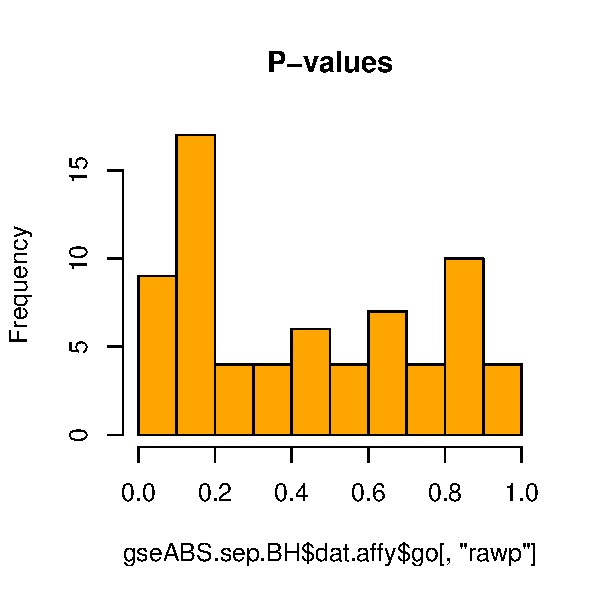
\includegraphics{Figures/plots-figure004}
\caption[\small P-value histogram]{\small
Histogram for p-values before multiple testing correction.
}
\label{fig:figure004}
\end{center}
\end{figure}

\newpage
Below is the code to produce the q-value histogram
shown in Figure~\ref{fig:figure005}:

\begin{figure}[htbp]
\begin{center}
\begin{Schunk}
\begin{Sinput}
> hist(gseABS.sep.BH$dat.affy$go[ , "BH"], nclass=10, col="orange",
+      main="Q-values")
\end{Sinput}
\end{Schunk}
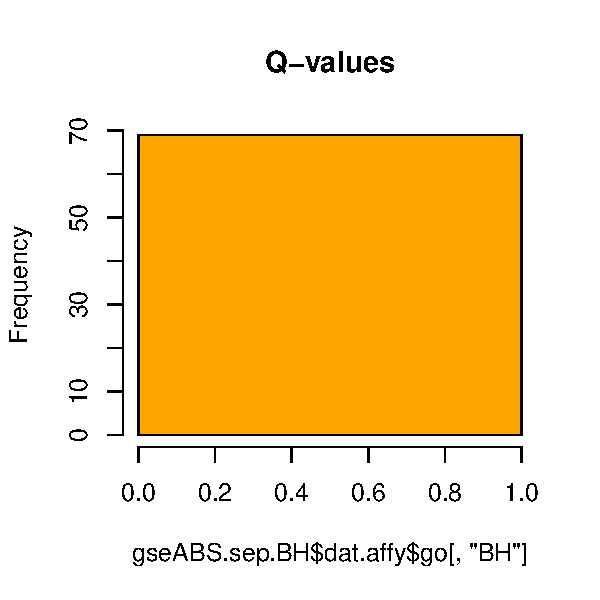
\includegraphics{Figures/plots-figure005}
\caption[\small P-value histogram]{\small
Histogram for q-values after multiple testing correction
with the Benjamini-Hochberg method.
}
\label{fig:figure005}
\end{center}
\end{figure}


\newpage
\section{Another example with a list of genes}
We will now use our function to perform GSA with a list of
autism candidate genes. This gene list is stored in the file
{\bf \texttt{"./myData/101symbols\_v02.txt"}}.
We will define a new function \Rcode{formatGeneList}
to prepare the data for the analysis.
We will compare our list against all the annotated
genes present in the genome (according to the information
contained in the \Rcode{org.Hs.eg.db}),
using the previously defined function based n the Fisher's Exact test.
First of all, however, we will read the least of genes in the {\R} session
and process the data to have them in the correct format.

\begin{Schunk}
\begin{Sinput}
> autismGenes <- read.table("myData/101symbols_v02.txt", sep="\t", header=TRUE,
+                           colClasses="character")
> str(autismGenes)
\end{Sinput}
\begin{Soutput}
'data.frame':	101 obs. of  1 variable:
 $ SYMBOL: chr  "ANKRD11" "AP1S2" "ARX" "ATRX" ...
\end{Soutput}
\end{Schunk}

The new function \Rcode{formatGeneList} will take
two lists of genes:
\begin{itemize}
\item The gene list of interest;
\item The "background" gene list (i.e. the "gene space");
\end{itemize}

As follows:

\begin{Schunk}
\begin{Sinput}
> formatGeneList <- function (geneList, allGenes) {
+   stats <- 1* allGenes %in% geneList
+   names(stats) <- allGenes
+   out <- list(GeneList = stats)
+ 	}
\end{Sinput}
\end{Schunk}

And now we can prepare the data:

\begin{Schunk}
\begin{Sinput}
> allGenes <- unique(unlist(as.list(org.Hs.egSYMBOL)))
> str(allGenes)
\end{Sinput}
\begin{Soutput}
 chr [1:43819] "A1BG" "NAT2" "ADA" ...
\end{Soutput}
\begin{Sinput}
> geneMembership <- formatGeneList(autismGenes$SYMBOL, allGenes)
> str(geneMembership)
\end{Sinput}
\begin{Soutput}
List of 1
 $ GeneList: Named num [1:43819] 0 0 0 0 0 0 0 0 0 0 ...
  ..- attr(*, "names")= chr [1:43819] "A1BG" "NAT2" "ADA" "CDH2" ...
\end{Soutput}
\begin{Sinput}
> table(geneMembership$GeneList)
\end{Sinput}
\begin{Soutput}
    0     1 
43718   101 
\end{Soutput}
\end{Schunk}

And now we can run the enrichment analysis:

\begin{Schunk}
\begin{Sinput}
> gseMyList <- runBatchGSE(dataList=geneMembership, fgsList=fgsList,
+ 				 absolute=FALSE, gseFunc=gseFunc, threshold=0.5)
\end{Sinput}
\end{Schunk}


Let's look at the results:

\begin{Schunk}
\begin{Sinput}
> str(gseMyList)
\end{Sinput}
\begin{Soutput}
List of 1
 $ GeneList:List of 2
  ..$ go  : Named num [1:200] 1 1 1 1 0.0451 ...
  .. ..- attr(*, "names")= chr [1:200] "GO:0071680.response to indole-3-methanol" "GO:0009081.branched-chain amino acid metabolic process" "GO:0045950.negative regulation of mitotic recombination" "GO:0044337.canonical Wnt receptor signaling pathway involved in positive regulation of apoptotic process" ...
  ..$ kegg: Named num [1:200] 1 0.00249 1 1 1 ...
  .. ..- attr(*, "names")= chr [1:200] "00061.Fatty acid biosynthesis" "04270.Vascular smooth muscle contraction" "00500.Starch and sucrose metabolism" "03320.PPAR signaling pathway" ...
\end{Soutput}
\begin{Sinput}
> str(gseMyList$GeneList$kegg)
\end{Sinput}
\begin{Soutput}
 Named num [1:200] 1 0.00249 1 1 1 ...
 - attr(*, "names")= chr [1:200] "00061.Fatty acid biosynthesis" "04270.Vascular smooth muscle contraction" "00500.Starch and sucrose metabolism" "03320.PPAR signaling pathway" ...
\end{Soutput}
\begin{Sinput}
> summary(gseMyList$GeneList$kegg)
\end{Sinput}
\begin{Soutput}
     Min.   1st Qu.    Median      Mean   3rd Qu. 
0.0000007 0.1423000 1.0000000 0.6710000 1.0000000 
     Max. 
1.0000000 
\end{Soutput}
\begin{Sinput}
> table(is.na(gseMyList$GeneList$kegg))
\end{Sinput}
\begin{Soutput}
FALSE 
  200 
\end{Soutput}
\begin{Sinput}
> table(gseMyList$GeneList$kegg < 0.01)
\end{Sinput}
\begin{Soutput}
FALSE  TRUE 
  181    19 
\end{Soutput}
\begin{Sinput}
> table(gseMyList$GeneList$go < 0.01)
\end{Sinput}
\begin{Soutput}
FALSE  TRUE 
  183    17 
\end{Soutput}
\end{Schunk}

And now we can correct for multiple testing:

\begin{Schunk}
\begin{Sinput}
> gseMyList.BH <- adjustPvalGSE(gseMyList)
> gseMyList.BH$GeneList$go[ gseMyList.BH$GeneList$go[, "BH"] < 0.01 , ]
\end{Sinput}
\begin{Soutput}
                                                                          rawp
GO:0045838.positive regulation of membrane potential              2.519385e-10
GO:0048011.nerve growth factor receptor signaling pathway         1.375639e-05
GO:0007275.multicellular organismal development                   2.053012e-35
GO:2000822.regulation of behavioral fear response                 3.146650e-05
GO:0006325.chromatin organization                                 4.419086e-06
GO:0051130.positive regulation of cellular component organization 1.775857e-09
GO:0044710.single-organism metabolic process                      6.202976e-06
GO:0002009.morphogenesis of an epithelium                         3.093646e-06
GO:0021953.central nervous system neuron differentiation          6.029012e-10
                                                                            BH
GO:0045838.positive regulation of membrane potential              2.519385e-08
GO:0048011.nerve growth factor receptor signaling pathway         3.439096e-04
GO:0007275.multicellular organismal development                   4.106025e-33
GO:2000822.regulation of behavioral fear response                 6.992555e-04
GO:0006325.chromatin organization                                 1.473029e-04
GO:0051130.positive regulation of cellular component organization 8.879283e-08
GO:0044710.single-organism metabolic process                      1.772279e-04
GO:0002009.morphogenesis of an epithelium                         1.237458e-04
GO:0021953.central nervous system neuron differentiation          4.019342e-08
\end{Soutput}
\begin{Sinput}
> gseMyList.BH$GeneList$kegg[ gseMyList.BH$GeneList$kegg[, "BH"] < 0.01 , ]
\end{Sinput}
\begin{Soutput}
                                             rawp
04720.Long-term potentiation         2.168670e-05
04510.Focal adhesion                 1.046100e-04
05211.Renal cell carcinoma           2.168670e-05
04514.Cell adhesion molecules (CAMs) 6.982789e-07
04150.mTOR signaling pathway         2.419609e-04
                                               BH
04720.Long-term potentiation         0.0014457802
04510.Focal adhesion                 0.0052305001
05211.Renal cell carcinoma           0.0014457802
04514.Cell adhesion molecules (CAMs) 0.0001396558
04150.mTOR signaling pathway         0.0096784341
\end{Soutput}
\end{Schunk}



\section{System Information}
Session information:

\begin{Schunk}
\begin{Sinput}
> sessionInfo()
\end{Sinput}
\begin{Soutput}
R version 3.0.0 (2013-04-03)
Platform: x86_64-apple-darwin10.8.0/x86_64 (64-bit)

locale:
[1] en_US.UTF-8/en_US.UTF-8/en_US.UTF-8/C/en_US.UTF-8/en_US.UTF-8

attached base packages:
[1] parallel  stats     graphics  grDevices
[5] utils     datasets  methods   base     

other attached packages:
 [1] GO.db_2.9.0          KEGG.db_2.9.1       
 [3] multtest_2.16.0      annotate_1.38.0     
 [5] org.Hs.eg.db_2.9.0   RSQLite_0.11.4      
 [7] DBI_0.2-7            AnnotationDbi_1.22.6
 [9] RTopper_1.6.0        limma_3.16.5        
[11] Biobase_2.20.0       BiocGenerics_0.6.0  
[13] BiocInstaller_1.10.3

loaded via a namespace (and not attached):
[1] IRanges_1.18.1  MASS_7.3-26    
[3] splines_3.0.0   stats4_3.0.0   
[5] survival_2.37-4 tools_3.0.0    
[7] XML_3.96-1.1    xtable_1.7-1   
\end{Soutput}
\end{Schunk}

\pagebreak
\section{References}
   \bibliographystyle{unsrt}
   \bibliography{GeneSetAnalysis}

\end{document}


